% \handouts
% \ifx\handouts\undefined
 \documentclass{beamer}
% \else
%\documentclass[xcolor=svgnames,handout]{beamer}
%\fi

\mode<presentation>
{
  \useoutertheme{miniframes}
  \setbeamercovered{transparent}
}

\setbeamertemplate{footline}[frame number]

\setbeamertemplate{blocks}[rounded][shadow=true]

%\usecolortheme{seahorse}
\usecolortheme{rose}
%\usepackage{pictex}

\usepackage{babel}
\usepackage[utf8]{inputenc}
\usepackage{times}
\usepackage[T1]{fontenc}
\usepackage{moreverb}
\newcommand{\code}[1]{\texttt{#1}}
\newcommand{\E}{\mathrm{E}}
\let\overbatim\verbatim
\let\endoverbatim\endverbatim
\newenvironment{vcode}%
{\bgroup\baselineskip=0.8\baselineskip\overbatim}%
{\endoverbatim\egroup}

%
%  TO THINK BEFORE 2019 LECTURE
%  
%  Bradford Hill criteria???
%  More on mediation analysis?
%  Show solution of the algorithm in the mediation case
%  Show a plot of the Egger approach?
%  (Still, the lecture should not be longer)
%  Check that all graphs are correct!
% 


\newcounter{demo}
\newcommand{\Demo}{\stepcounter{demo}\frametitle{Demo \arabic{demo}}}

\title{Some topics on causal inference} 

\author{Krista~Fischer}

\institute[TY] % (optional, but mostly needed)
{
   Estonian Genome Center, University of Tartu, Estonia
}

\date[Lyon 2018] % (optional)
{Statistical Practice in Epidemiology, Lyon 2018}


\begin{document}

\begin{frame}
  \titlepage
\end{frame}

\section*{Outline}
\begin{frame}
\tableofcontents
\end{frame}

\section{How to define a causal effect?}

\begin{frame}
  \frametitle{Statistical associations vs causal effects in epidemiology}
  \begin{block}{}
  Does the exposure (smoking level, obesity, etc) have a \alert<2>{causal effect} on the outcome (cancer diagnosis, mortality, etc)?
  \end{block}
is not the same question as   
 \begin{block}{}
  Is the exposure \alert<3>{associated} with the outcome?
  \end{block}
 Conventional statistical analysis will answer the second one, but not necessarily the first. 
%  \end{itemize}
\end{frame}

\begin{frame}
  \frametitle{What is a causal effect?}
  
 \emph{There is more than just one way to define it.}
 
 A causal effect may be defined:
  \begin{itemize}
  \item At the \alert<1>{individual level}: \\
  \alert<1>{\textit{Would my cancer risk be different if I were a (non-)smoker?}}
  \item At the \alert<2>{population level}: \\
  \alert<2>{\textit{Would the population cancer incidence be different if the prevalence of smoking were different?}}
  \item At the \alert<3>{\textit{exposed subpopulation level}}: \\
  \alert<3>{Would the cancer incidence in smokers be different if they were nonsmokers?}
  \end{itemize}
\alert<4>{
None of these questions is ``mathematical'' enough to provide a mathematically correct definition of causal effect 
}
\end{frame}



\begin{frame}
\frametitle{Causal effects and counterfactuals}
\begin{itemize}
\item Defining the causal effect of an observed exposure always involves some \alert<1>{counterfactual} (what-if) thinking.
\item The individual causal effect can be defined as the difference 
 \[Y(X=1) - Y(X=0)\].
where $Y(1)=Y(X=1)$ and $Y(0)=Y(X=0)$ are defined as individual's \alert<2>{potential (counterfactual)} outcomes if this individual's exposure level $X$ were \alert<2>{set} to 1 or 0, respectively. 
\item Sometimes people (e.g J. Pearl) use the \alert<3>{``do''} notation to distinguish counterfactual variables from the observed ones: $Y(do(X=1))$ and $Y(do(X=0))$.     
\end{itemize}
\end{frame}

\begin{frame}
  \frametitle{The ``na\"ive'' association analysis}
  {\small  \begin{itemize}
  \item With a binary exposure $X$, compare average outcomes in exposed and unexposed populations:
  \[E(Y|X=1) - E(Y|X=0)\]
  \textit{Is cancer incidence different in smokers and nonsmokers?}
  \item But mostly:
  \[E(Y|X=1) \ne E(Y(1))\]
  \textit{Cancer risk in smokers is not the same as the potential cancer risk in the population if everyone were smoking}
  \item Similarly:
  \[E(Y|X=0) \ne E(Y(0))\]
 % \textit{Cancer risk in nonsmokers is not the same as the potential cancer risk in the population if there were no %smokers}
  \item In most cases there is always some \alert{unobserved confounding} present and therefore the
   na\''ive analysis does not provide causal effect estimates.  
  \end{itemize}}
\end{frame}

\begin{frame}
\frametitle{Counterfactual outcomes in different settings}
\begin{itemize}
\item \alert<1>{Randomized trials}: probably the easiest setting to imagine $Y(X)$ for different $X$
\item \alert<2>{``Actionable'' exposures}: smoking level, vegetable consumption, \ldots -- potential interventions may alter exposure levels in future.
\item \alert<3>{Non-actionable exposures}: e.g genotypes. It is difficult to ask \emph{``What if I had different genes?''}. Still useful concept to formalize genetic effects (heritability, attributable risk).
\item \alert<4>{Combinations}: With X-- a behavioral intervention level, Z--smoking level and Y--a disease outcome, one could formalize the effect of intervention on outcome by using $Y(X, Z(X))$
\end{itemize}
\end{frame}


\begin{frame}
 \frametitle{Classical/generalized regression estimates vs  causal effects?}
 \begin{itemize}
 \item In the presence of confounding, regression analysis provides a biased estimate for the true causal effect
\item To reduce such bias, one needs to collect data on most important confounders and adjust for them
\item However, too much adjustment may actually introduce more biases   
\item Causal graphs (Directed Acyclic Graphs, DAGs) may be extremly helpful in identifying the optimal set of adjustment variables
\end{itemize}
 \end{frame}


\section{Causal graphs, confounding and adjustment}

\begin{frame}
  \frametitle{Adjustment for confounders I}
 ``Classical'' confounding: situation where third factors  Z influence both, X and Y \\[-0.2cm]
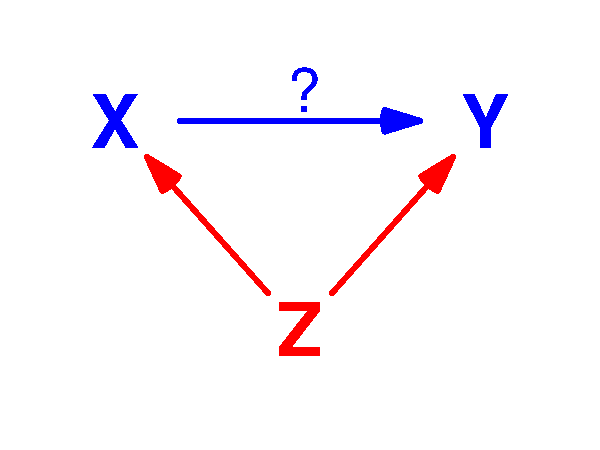
\includegraphics[width=4cm]{confound}\\[-0.3cm]
For instance, one can assume: \ $X = Z + U$ \ and \ $Y = Z + V$, \\
where $U$ and $V$ are independent of  $Z$. \pause

$X$ and $Y$ are independent, conditional on $Z$, but marginally dependent.

\alert{One should adjust the analysis for $Z$, by fitting a regression model for $Y$ with covariates
 $X$  and $Z$.} There is a causal effect between $X$ and $Y$, if the effect of $X$ is present in such model.
\end{frame}

\begin{frame}
\frametitle{Adjustment may sometimes make things worse}
Example: the effect of X and Y on  Z:   \\[-0.2cm]
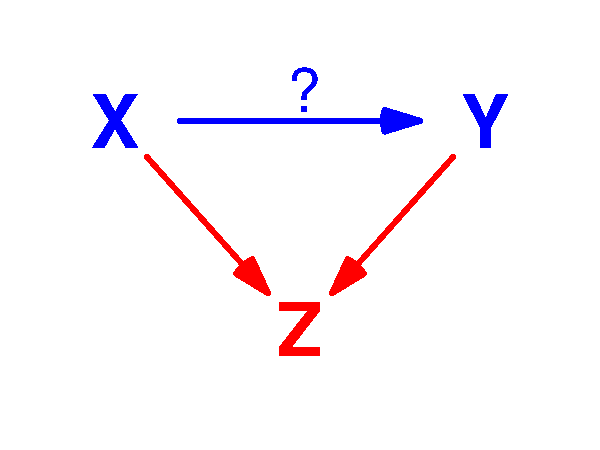
\includegraphics[width=4cm]{wrongadjust}\\[-0.3cm]
A simple model may hold:
$Z = X + Y + U$, \\
where $U$ is independent of $X$ and $Y$. \\
Hence $Y = Z - X - U$.

\pause
\alert<1>{We see the association between $X$ and $Y$ only when the ``effect'' of  $Z$ has been taken into account.
But this is not the causal effect of $X$ on $Y$.}

\alert<2>{One should NOT adjust the analysis for $Z$!}
\end{frame}

\begin{frame}
\frametitle{More possibilities: mediation}
Example: the effect of X on Y is (partly) \alert{mediated} by  Z:   \\[-0.2cm]
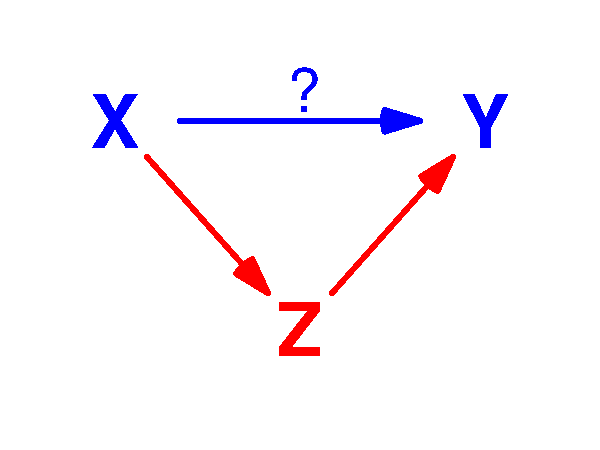
\includegraphics[width=4cm]{mediation}\\[-0.3cm]

$Y = X + Z + U$, \\

\pause
If you are interested in the \alert{total effect} of $X$ on $Y$ -- don't adjust for $Z$! \\

\pause
If you are interested in the \alert{direct effect} of $X$ on $Y$ -- adjust for $Z$. (Only if the $Z$-$Y$ association is unconfounded)
\end{frame}

%\begin{frame}
%\frametitle{Even more possibilities: reverse causation}
%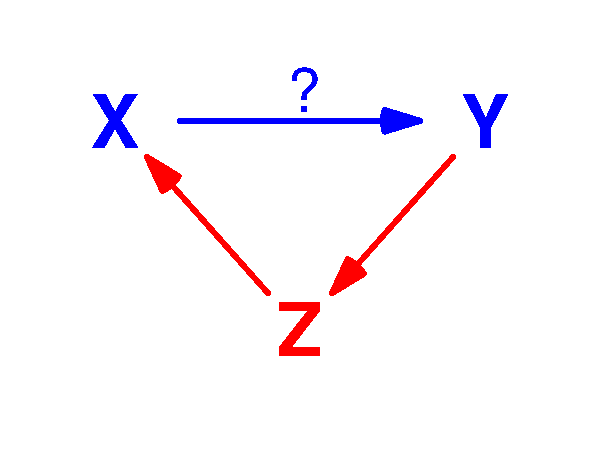
\includegraphics[width=4cm]{revcaus}\\[-0.3cm]

%Now the graph is not any more acyclic -- it is not a DAG!  Can occur by omitting a temporal component. 
%One should modify the graph (and data collection procedure) to enable valid causal inference.     

%\end{frame}


\begin{frame}
 Actually there might be a complicated system of
causal effects:

{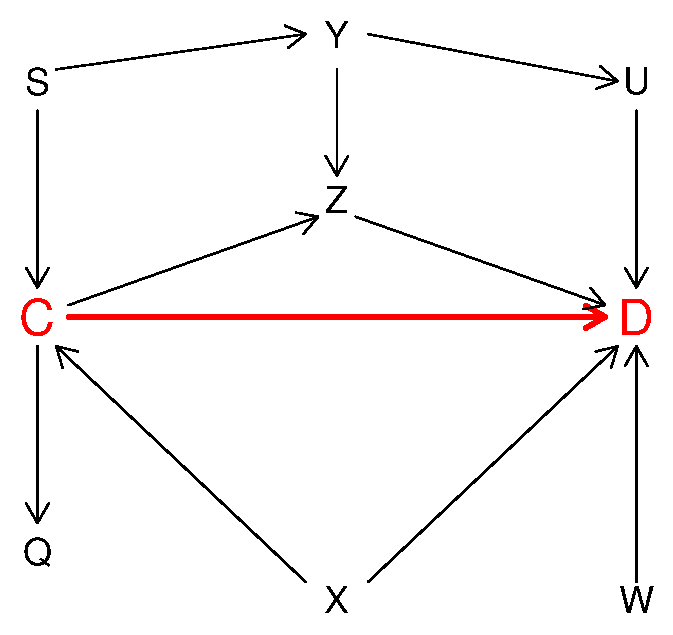
\includegraphics[width=0.5\textwidth]{keeruline2}}\\
{\small  C-smoking; D-cancer \\
Q, S, U, W, X, Y, Z - other factors that influence cancer risks
and/or smoking (genes, social background, nutrition, environment,
personality, \ldots)}
\end{frame}

\begin{frame}
 \emph{To check for confounding,}

\begin{enumerate}
\item Sketch a causal graph
\item
 Remove all arrows corresponding to the causal effect of interest
 (thus, create a graph where the causal null-hypothesis would hold).
 \item Remove all nodes (and corresponding edges) except
 those contained in the exposure ($C$) and outcome ($D$) variables and their (direct or indirect)
ancestors. 
\item
Connect by an undirected edge every pair of nodes that both
share a common child and are not already connected by a
directed edge. 
\begin{itemize}
\item If now $C$ and $D$ are still associated, we say that the $C-D$
association is confounded  
\item Identify the set of nodes that need to be deleted to separate $C$ and $D$ --  inferences conditional
on these variables give unconfounded estimates of the causal effects.
\end{itemize}
\end{enumerate}
\end{frame}

\begin{frame}
\frametitle{Example: mediation with confounding}
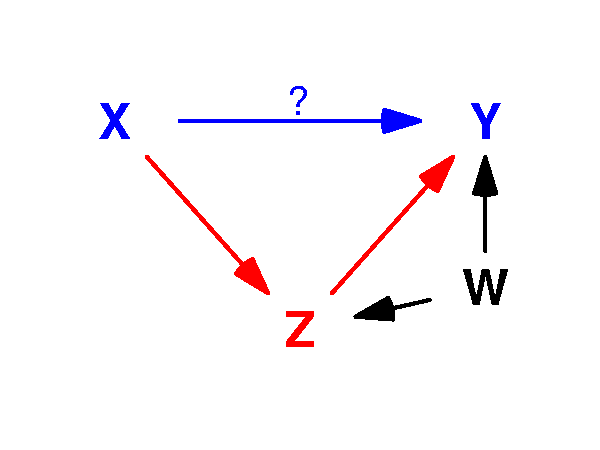
\includegraphics[width=6cm]{mediation_conf}\\[-0.3cm]

Follow the algorithm to show that one should adjust the analysis for $W$. If $W$ is an unobserved confounder, no valid causal inference is possible in general. However, the total effect of $X$ on $Y$ is estimable.

\end{frame}

\section{Causal models for observational data}
\subsection{Instrumental variables estimation and Mendelian randomization}
\begin{frame}
  \frametitle{``Mendelian randomization'' -- genes as Instrumental Variables}
    \begin{itemize}
  \item \alert<1>{Most of the exposures of interest in chronic disease epidemiology cannot be randomized.}
  \item \alert<2>{Sometimes}, however, nature will randomize for us: \alert<2>{there is a SNP (Single nucleotide polymorphism, a DNA marker) that affects the exposure of interest, but not directly the outcome.} 
  \item Example: a SNP that is associated with the enzyme involved in alcohol metabolism, genetic lactose intolerance, etc. 
  \end{itemize}
However, the crucial assumption that the SNP cannot affect outcome in any other way than throughout the exposure, cannot be tested statistically!
\end{frame}


\begin{frame}
 \frametitle{General instrumental variables estimation}
A causal graph with exposure $X$, outcome $Y$, confounder $U$ and an \emph{instrument} $Z$:\\
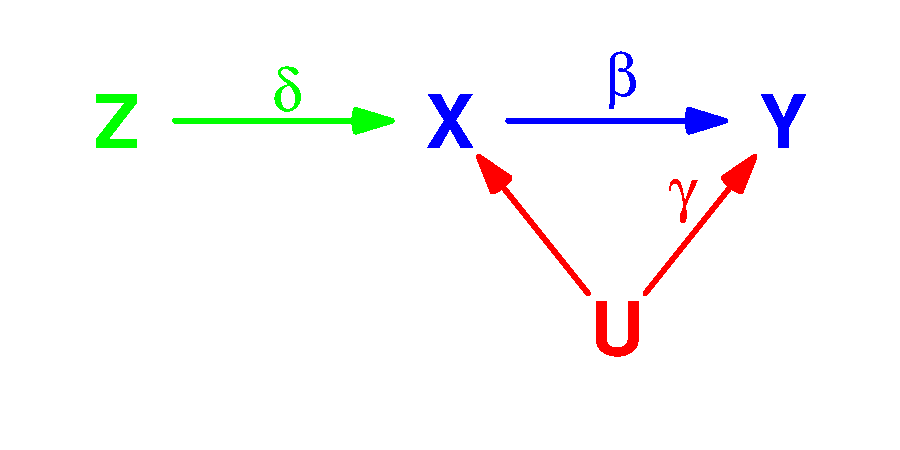
\includegraphics[width=6cm]{instvar} \\
Simple regression will yield a biased estimate of the causal effect of $X$ on $Y$, as the graph implies:
\[ Y= \alpha_y + \beta X + \gamma U +\epsilon,  \  \E(\epsilon|X,U)=0 \]
so $\E(Y|X)= \alpha_y + \beta X + \gamma \E(U|X)$. \\
Thus the coefficient of $X$ will also depend on $\gamma$ and the association between $X$ and $U$. 
\end{frame}

\begin{frame}
 \frametitle{General instrumental variables estimation}
\mbox{ }\\[-1cm]
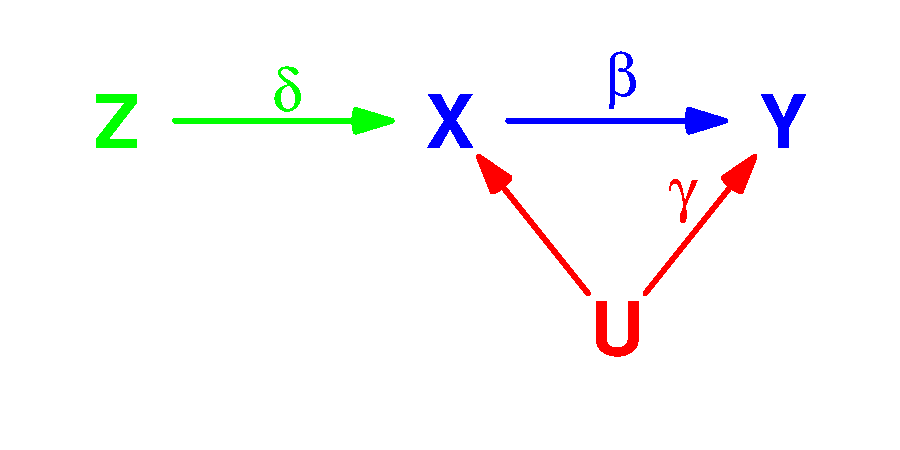
\includegraphics[width=6cm]{instvar} \\[-0.5cm]
\[ Y= \alpha_y + \beta X + \gamma U +\epsilon,  \  \E(\epsilon|X,U)=0 \]
\mbox{ }\\
\textcolor{green}{How can Z help?} \\
\pause
If $ \ \E(X|Z)=\alpha_x + \delta Z, \ $  we get  \pause
\[
\E(Y|Z) = \alpha_y + \beta E(X|Z) + \gamma E(U|Z)  =   \alpha_y + \beta(\alpha_x + \delta Z) = \alpha_y^* + \beta\delta Z. 
\]
\pause As $\delta$ and $\beta\delta$ are estimable, also $\beta$ becomes estimable. 
\end{frame}

\begin{frame}
 \frametitle{General instrumental variables estimation}
\mbox{ }\\[-1cm]
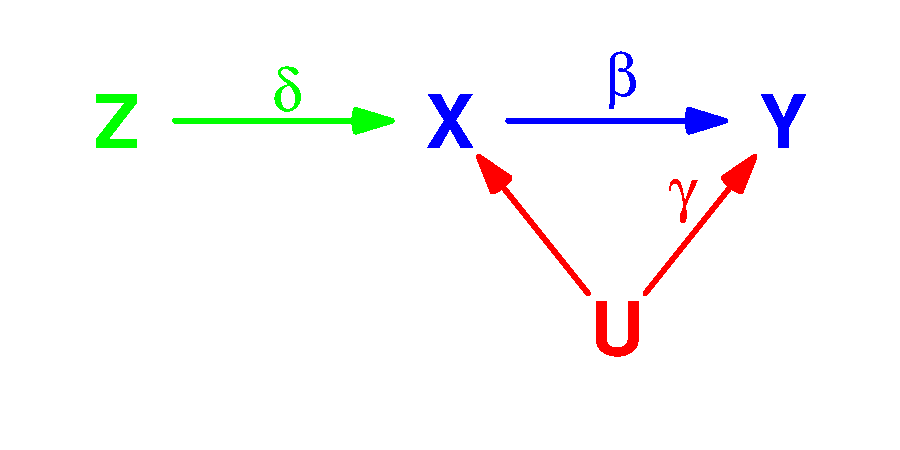
\includegraphics[width=6cm]{instvar}\\
\begin{enumerate}
\item Regress $X$ on $Z$, obtain an estimate $\hat{\delta}$
\item Regress $Y$ on $Z$, obtain an estimate $\hat{\delta\beta}$ 
\item Obtain $\hat{\beta} = \frac{\hat{\delta\beta}}{\hat{\delta}}$
\item \alert{Valid, if Z is not associated with $U$ and does not have any effect on $Y$ (other than mediated by $X$)} 
\small
\item Standard error estimation is more tricky -- use for instance \code{library(sem)}, function \code{tsls()}.
\end{enumerate}
\normalsize
\end{frame}
\begin{frame}
 \frametitle{Mendelian randomization example}
 FTO genotype, BMI and Blood Glucose level (related to Type 2 Diabetes risk; Estonian Biobank, n=3635, aged 45+)
\mbox{ }\\[-0.5cm]
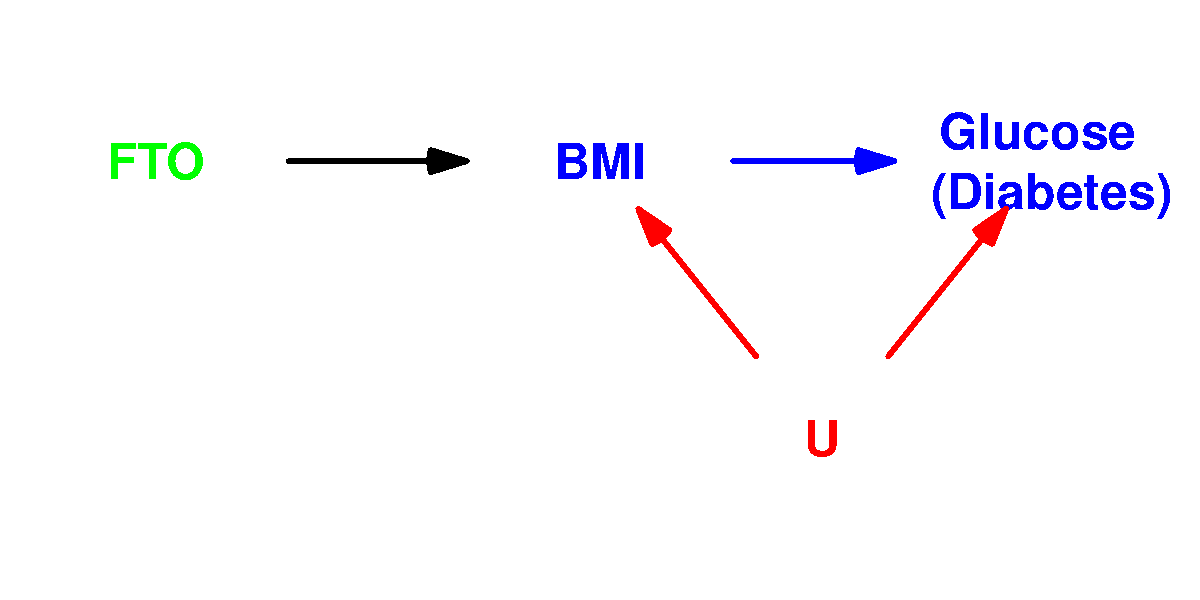
\includegraphics[width=7cm]{mendrand}\\[-0.5cm]
\begin{itemize}
\item Average difference in Blood Glucose level (Glc, mmol/L) per BMI unit is estimated as 0.085 (SE=0.005)
\item Average BMI difference per FTO risk allele is estimated as 0.50 (SE=0.09)
\item Average difference in Glc level per  FTO risk allele is estimated as 0.13 (SE=0.04)
\item \alert{ Instrumental variable estimate of the mean Glc difference per BMI unit is 0.209 (se=0.078)}
\end{itemize}
\end{frame}

\begin{frame}[fragile]
\frametitle{IV estimation in R (using \code{library(sem)}):}
\small
\begin{vcode}
> summary(tsls(Glc~bmi, ~fto,data=fen),digits=2)

 2SLS Estimates

Model Formula: Glc ~ bmi

Instruments: ~fto

Residuals:
   Min. 1st Qu.  Median    Mean 3rd Qu.    Max. 
-6.3700 -1.0100 -0.0943  0.0000  0.8170 13.2000 

            Estimate Std. Error t value Pr(>|t|)   
(Intercept)   -1.210      2.106    -0.6    0.566   
bmi            0.209      0.078     2.7    0.008 **
\end{vcode}
\normalsize
\end{frame}

\begin{frame}[fragile]
\frametitle{IV estimation: can untestable assumptions be tested?}
\small
\begin{vcode}
> summary(lm(Glc~bmi+fto,data=fen))
Coefficients:
            Estimate Std. Error t value Pr(>|t|)    
(Intercept) 1.985  0.106   18.75   <2e-16 ***
bmi         0.088  0.004   23.36   <2e-16 ***
fto         0.049  0.030    1.66    0.097 .  

For Type 2 Diabetes:
> summary(glm(t2d~bmi+fto,data=fen,family=binomial))
Coefficients:
             Estimate Std. Error z value Pr(>|z|)    
(Intercept) -7.515   0.187  -40.18   <2e-16 ***
bmi          0.185   0.006   31.66   <2e-16 ***
fto          0.095   0.047    2.01    0.044 *  
\end{vcode}
\normalsize
Does FTO have a direct effect on Glc or T2D?  \\
\alert{A significant FTO effect would not be a proof here (nor does non-significance prove the opposite)! (WHY?)}
\end{frame}


\begin{frame}
\frametitle{Can we test pleiotropy?}
A na\"{i}ve approach would be to fit a linear regression model for $Y$, with both $X$ and $G$ as covariates.
\\
But in this case we estimate: 
\[
\E(Y|X, G) = \mbox{const} + \beta_{pl} G + \beta  X + \gamma \E(U|X, G).  
\]
It is possible to show that $U$ is not independent of neither $X$ nor $G$ -- therefore, the coefficient of $G$ in the resulting model would be nonzero even if $\beta_{pl}=0$.

\alert{Therefore there is no formal test for pleiotropy possible in the case of one genetic instrument -- only biological arguments could help to decide, whether assumptions are likelt to be fulfilled} \\
In the case of \emph{multiple genetic instruments} and \emph{meta-analysis}, sometimes the approach of \emph{Egger regression} can be used (Bowden et al, 2015). But even that is not an assumption-free method!
\end{frame}

\section{Summary and references}
\begin{frame}
\frametitle{Summary}
\begin{itemize}
\item There is no unique definition of ``the causal effect'' 
\item The validity of any causal effect estimates depends on the validity of the underlying assumptions.
\item Adjustment for other available variables may remove (some) confounding, but it may also create more confounding. \alert{Do not adjust for variables that may themselves be affected by the outcome.}   
\item Instrumental variables approaches can be helpful, but beware of assumptions! 
\end{itemize}
\end{frame}



\section{References}
\begin{frame}
\frametitle{Some references}
{\small
\begin{itemize}
\item A webpage by Miguel Hernan and Jamie Robins: 
\href{http://www.hsph.harvard.edu/miguel-hernan/causal-inference-book/}{http://www.hsph.harvard.edu/miguel-hernan/causal-inference-book/}
\item An excellent overview of Mendelian randomization: \\
Sheehan, N., Didelez, V., Burton, P., Tobin, M., Mendelian Randomization and Causal Inference in Observational Epidemiology, PLoS Med. 2008 August; 5(8). 
\item A way to correct for pleiotropy bias: \\
Bowden J, Davey Smith G, Burgess S, Mendelian randomization with invalid instruments: effect estimation and bias detection through Egger regression. Int J Epidemiol. 2015 Apr;44(2):512-25.
\item \ldots and how to interpret the findings (warning against overuse): \\ Burgess, S., Thompson, S.G., Interpreting findings from Mendelian randomization using the MR-Egger method, Eur J Epidemiol (2017). 
\end{itemize}}
\end{frame}
\end{document}

